\section{Wednesday 09/04/2024}
\subsection{P, NP, NP-complete, and NP-hard}
\begin{figure}[htbp]
  \centerline{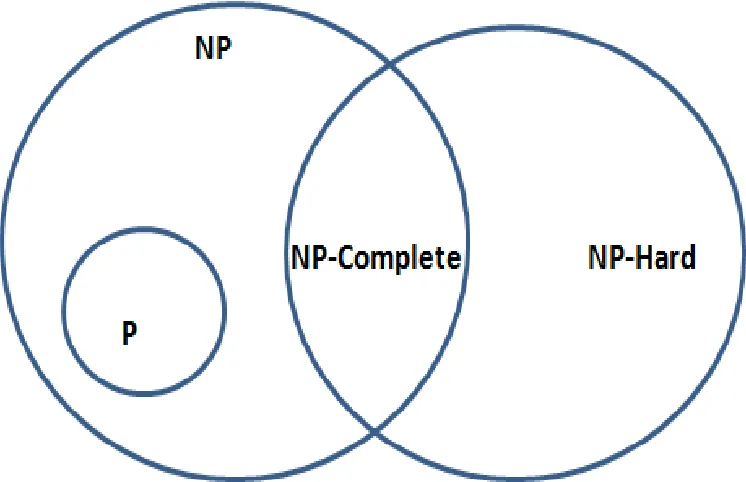
\includegraphics[width=0.6\textwidth]{images/p_venn_diagram.png}}
\end{figure}

\framebox[\linewidth]{
    \begin{minipage}{\dimexpr\linewidth-2\fboxsep-2\fboxrule\relax}
        A \textbf{problem} is a function $F : I \to B$, where I is the set of instances encoded as strings of characters and B is the set of problem outputs.
    \end{minipage}
}

A mapping from I to B by taking in the input parameters of what the specific problem actually entails, and then the solution or answer is parametrized by B.
\\ \\
For example, linear programming in $\mathbb{R}^{mxn}$ is a problem where the instance parameters are $(m,n,A,c,b)$ and the output $B$ is the optimal solution found to the objective function.
\\ \\ 
Another example, making a decision takes in an instance $I$ and outputs a decision of yes or no.
\begin{equation}
  I = \textit{Problem-specific information parameters}, B \in (yes, no)
\end{equation}

\subsubsection{Turing machine}
A turing machine is a model of how a computer processes a program. There is a \textit{tape} and \textit{finite-state controller}  
\begin{itemize}
  \item \textbf{Tape}: A memory unit divided into tape cells. Each tape cell stores one symbol chosen from a finite set of symbols. The tape head is the sole cell currently processed by the controller. 
  \item \textbf{Finite-state controller}: A collection of finite states and rules where at each time step, the controller takes an action of erase, move, update cell, and update state.
\end{itemize}

There is only one unique rule applied for each symbol-state combination
\\ \\ 
A turing machine is said to be able to solve a problem $F : I \to B $, if given any instance $x \in I$, the turing machine eventually produces the solution $B$ and stops.
\\ \\
My understanding of this is that a turing machine has a controller that goes and selects individual cells based off of the symbol and then makes an action to change the state based off of a set of symbol-state pairs.

\subsubsection{P-problem}
\framebox[\linewidth]{
    \begin{minipage}{\dimexpr\linewidth-2\fboxsep-2\fboxrule\relax}
       The class P of problems is defined to be those problems $ F: I \to {yes,no}$ such that a Turing machine M can compute F, and the number of steps required by M for this computation is bounded by $p(n)$ where $p$ is a polynomial and $n$ is the length of the input. 
    \end{minipage}
}
\\ \\ 
In other words, a problem P can be solved in polynomial time by a turing machine.
\\ \\ 
F is a decision problem
\\ \\ 
\textbf{NP problem}: Problems whose solution, if it is "yes", have proofs verifiable in polynomial time by a deterministic Turing machine.
\\ \\ 
P problems can be solved in polynomial time, NP problems are problems that can be verified in polynomial time. A non-deterministic Turing machine would be able to solve an NP problem in polynomial time. \textit{A non-deterministic Turing machine is defined as the relaxation of the "unique rule per symbol-state" constraint.} 
\\
For example, in the exercise done in class, instead of having the unique rule of "if no one is to the right, say 'yes'", you could have a non-deterministic rule where you have a 50\% chance of saying 'no' or 'yes'. Putting randomness in the rule would make it a non-deterministic machine.

\subsubsection{NP-complete}
\framebox[\linewidth]{
    \begin{minipage}{\dimexpr\linewidth-2\fboxsep-2\fboxrule\relax}
       A decision problem $F : I \to {yes, no}$ can be polynomial transformed into another decision problem $ G : I^\prime \to {yes, no}$ if there exists a function $f : I \to I^\prime$. The function f can be computed by a polynomial-time Turing machine, and $f$ has the property that $F(x) = yes \iff G(f(x)) = yes$ 
    \end{minipage}
}
\\ \\
\framebox[\linewidth]{
    \begin{minipage}{\dimexpr\linewidth-2\fboxsep-2\fboxrule\relax}
      Suppose $F : I \to {yes, no}$ is a decision problem that lies in NP, and suppose that every problem in NP can be polynomially transformed to F . Then, F is said to be NP-complete
    \end{minipage}
}
\\ \\ 
An algorithm can solve all NP problem efficiently if it can solve an NP-complete problem efficiently. If it solves an NP-complete problem, that means it is able to transform a problem into an NP problem.

\section{Friday 09/06/2024}
I did not attend this day so just notes over the slides.
\subsection{NP-hard}
\subsubsection{Definitions}
\framebox[\linewidth]{
    \begin{minipage}{\dimexpr\linewidth-2\fboxsep-2\fboxrule\relax}
        We say that a Turing machine can use $F$ as an \textbf{oracle} if $M$ is augmented with the following capability: $M$ can compute $F(x)$ from $x$ in one step.
    \end{minipage}
}
\\ \\ 
\framebox[\linewidth]{
    \begin{minipage}{\dimexpr\linewidth-2\fboxsep-2\fboxrule\relax}
        We say that a problem $G$ is \textbf{Cook-reducible} to problem $F$ (aka, polynomial-time Turing reducible) if $G$ can be computed in polynomial time by a Turing machine that uses $F$ as an oracle.
    \end{minipage}
}
\\ \\ 
\framebox[\linewidth]{
    \begin{minipage}{\dimexpr\linewidth-2\fboxsep-2\fboxrule\relax}
        A problem $F$ is said to be \textbf{NP-hard} if an NP-complete problem is Cook-reducible to F.
    \end{minipage}
}
\\ \\ 
\subsubsection{Quadratic problem}
\textbf{General quadratic programming:}
\begin{itemize}
  \item Given symmetric matrix $ H \in \mathbb{R}^{n x n}, \text{ matrix } A \in \mathbb{R}^{m x n}, \text{ and vectors } \textbf{b,c} \in \mathbb{R}^n $
  \item Solve
\end{itemize}

\begin{equation}
  \label{GQP}\tag{GQP}
  \begin{aligned}
    \min \textbf{x}^T H \textbf{x} + \textbf{c}^T \textbf{x} \\
    s.t. A \textbf{x} \geq \textbf{b}
  \end{aligned}
\end{equation}


